\documentclass[onecolumn, draftclsnofoot,10pt, compsoc]{IEEEtran}
\usepackage{graphicx}
\usepackage{url}
\usepackage{setspace}
\usepackage{caption}

\usepackage{geometry}
\geometry{textheight=9.5in, textwidth=7in}


% 1. Fill in these details
\def \CapstoneTeamName{		    Nitro Chatbot}
\def \CapstoneTeamNumber{		63}
\def \GroupMemberOne{			Jack Barnes}
\def \GroupMemberTwo{			Sarun Pitaksuteephong}
\def \GroupMemberThree{			Cheng Xie}
\def \CapstoneProjectName{		ChatBot for Load Balancer Infrastructure}
\def \CapstoneSponsorCompany{	OSU Information Services}
\def \CapstoneSponsorPerson{	Stacy Brock}

% 2. Uncomment the appropriate line below so that the document type works
\def \DocType{	%Problem Statement
				%Requirements Document
				%Technology Review
				Design Document
				%Progress Report
				}

\newcommand{\NameSigPair}[1]{\par
\makebox[2.75in][r]{#1} \hfil 	\makebox[3.25in]{\makebox[2.25in]{\hrulefill} \hfill		\makebox[.75in]{\hrulefill}}
\par\vspace{-12pt} \textit{\tiny\noindent
\makebox[2.75in]{} \hfil		\makebox[3.25in]{\makebox[2.25in][r]{Signature} \hfill	\makebox[.75in][r]{Date}}}}
% 3. If the document is not to be signed, uncomment the RENEWcommand below
\renewcommand{\NameSigPair}[1]{#1}

%%%%%%%%%%%%%%%%%%%%%%%%%%%%%%%%%%%%%%%
\begin{document}
\begin{titlepage}
    \pagenumbering{gobble}
    \begin{singlespace}
    	% 4. If you have a logo, use this includegraphics command to put it on the coversheet.
    	%\includegraphics[height=4cm]{logo-small-notext.png}
        \hfill 
        \par\vspace{.2in}
        \centering
        \scshape{
            \huge CS Capstone \DocType \par
            {\large\today}\par
            \vspace{.5in}
            \textbf{\Huge\CapstoneProjectName}\par
            \vfill
            %\includegraphics[height=8cm]{logo-small-notext.png}
            \vfill
            {\large Prepared for}\par
            \Huge \CapstoneSponsorCompany\par
            \vspace{5pt}
            {\Large\NameSigPair{\CapstoneSponsorPerson}\par}
            {\large Prepared by }\par
            Group\CapstoneTeamNumber\par
            % 5. comment out the line below this one if you do not wish to name your team
            \CapstoneTeamName\par 
            \vspace{5pt}
            {\Large
                \NameSigPair{\GroupMemberOne}\par
                \NameSigPair{\GroupMemberTwo}\par
                \NameSigPair{\GroupMemberThree}\par
            }
            \vspace{20pt}
        }
        \begin{abstract}
        % 6. Fill in your abstract
            This document outlines the entire design of the software project known as Nitro Chatbot, which is the proposed solution to the project proposal "ChatBot for Load Balancer Infrastructure".
            This document serves as an informative document for the development team to communicate a detailed blueprint of the proposed design to the stakeholders.
            Nitro Chatbot is comprised of 3 main components (Chatbot, Relay, Deployment) that work in unison to provide a solution.
            The chatbot (deployed to AWS) will connect to Microsoft Teams, accept command input, authenticate users, forward requests to the relay, receive replies and display them to the user.
            The relay will await requests from the chatbot, forward them to the load balancer, and return the response to the chatbot.
            Finally, the deployment module describes the continuous integration/continuous deployment (CI/CD) pipeline used to rapid and reliable development.
        \end{abstract}     
    \end{singlespace}
\end{titlepage}
\newpage
\pagenumbering{arabic}
\tableofcontents
% 7. uncomment this (if applicable). Consider adding a page break.
\listoffigures
\listoftables
\clearpage
\textbf{Change History}\par

\begin{tabular}{ p{1in} p{1in} p{4in} }
 \textbf{Revision} & \textbf{Date} & \textbf{Changes} \\
 \hline
 1.0 & 11/25/2019 
 & - \\
 \hline
 1.1 & 12/03/2019 
 & Both figures have been updated to the latest versions. Language has be clarified that users must use direct messages to send commands to the chatbot. User commands have been consolidated into a table. Deployment have been changed to an EC2 instance to meet the availability requirement. Administrative specifications clarified. \\
 \hline
\end{tabular}

\clearpage

% 8. now you write!
\section{Introduction}

\subsection{Purpose}
Nitro Chatbot will provide a chatbot interface for users to query the status of their load balanced resources within the Oregon State University network.
Users with the correct permissions will be able to quickly access the status and perform common configuration tasks on the University's load balancer, a Citrix NetScaler.

\subsection{Scope}
Two primary software components will need to be developed.
The first component is the chatbot that will accept commands from a user.
The first component is known as the chatbot, but may also be referenced as the front-end or the user interface (UI), as it provides both of these functions for the software system.
The second component software will act as a relay, receiving requests from the chatbot, sending commands to the load balancer from within the network and then returning the results to the chatbot.
The relay is also known as the back-end as it performs actions out of view of the user.
The relay will maintain authentication for active users and perform the direct interaction with the load balancer API (Application Program Interface).
This will allow the chatbot to provide quick access to the status and configuration options for the server pools that the user's manage.

\subsection{Intended Audience}
Users of this chatbot will be system administrators who manage server pools at Oregon State University. They have ONID (OSU Network ID) accounts.
They have a high-level of technical understanding and are familiar with command line interfaces.
The targeted user base is approximately 2 dozen people.

\subsection{Definitions}
\underline{Botkit Framework}: An open-source developer tool for building chatbot that also allows custom integration for major messaging platforms. Has direct access to platform APIs. It is owned by Microsoft \cite{framework}.
\\\underline{Chatbot}: A chatbot is a piece of software that conducts a conversation via auditory or textual methods \cite{chatbot}.
\\\underline{Citrix NetScaler}: A an application delivery controller made by Citrix that load balances to make sure that applications can be run as smooth as possible \cite{netscaler}.
\\\underline{Duo}: It is a vendor for cloud-based two-factor authentication service. It can be integrated with any website, VPN (Virtual Private Network), and cloud services \cite{duo}.
\\\underline{Load Balancer}: Load balancer is a reverse proxy that distributes network or application traffic across the server pool. This will increase the efficiency, maintainability, and, speed of the server pool. 
\\\underline{NITRO API}: The NetScaler NITRO protocol allows you to configure and monitor the NetScaler appliance programmatically by using Representational State Transfer (REST) interfaces \cite{citrixnitro}.
\\\underline{ONID}: Oregon State University ID used for identification
\\\underline{REST}: Representational State Transfer. It is a software architect style that defines what could be used for creating web services. The main constraint are the client that uses the API and the resources that the API can provide information to \cite{restphd} \cite{rest}.  
\\\underline{Server Pool}: An autonomous region that contains physical servers. It is a simplified unified view where virtual machines are located \cite{pools}.

\section{System Overview}
\begin{figure}[h]
    \centering
    \captionsetup{format=hang,justification=raggedright,margin=2cm}
    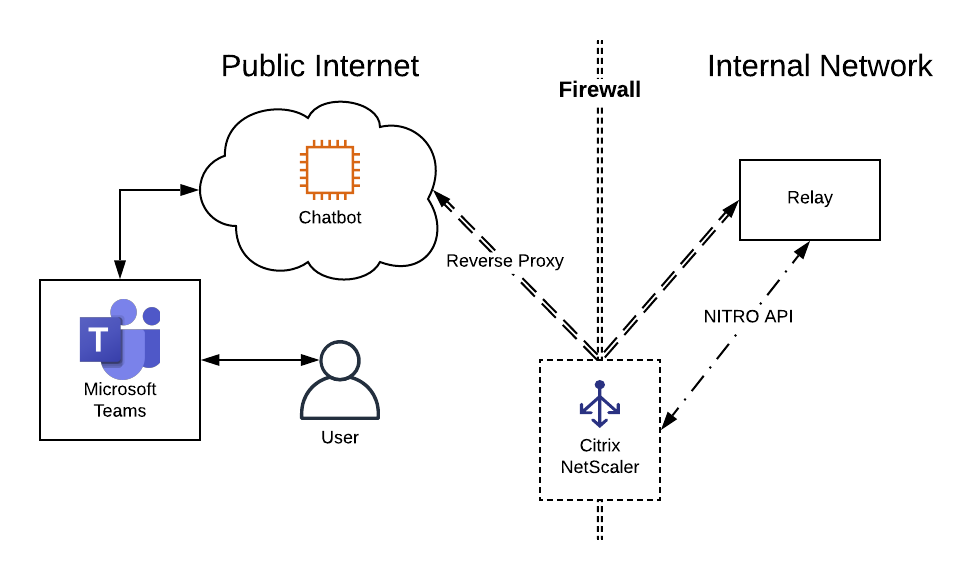
\includegraphics[height=6cm]{overview.png}
    \caption[Basic overview of the chatbot]{Basic overview of the chatbot, and how it will allow users access to load balancer configurations.}
    \label{fig:NetScaler Chatbot}
\end{figure}
\subsection{System Design}
Nitro Chatbot is comprised of 3 main components (chatbot, relay, deployment) that work in unison.

The first component, chatbot, is a piece of software written in Node.js.
It serves as the User Interface (UI) and as the front-end.
It will connect to Microsoft Teams, receive commands from the user, authenticate them, forward requests to the relay, and display responses from the relay.

The second component, relay, is a piece of software that is written in Node.js.
The relay serves as the back-end of the software system.
It receives requests from the chatbot, formats and forwards them to the Citrix NetScaler (a load balancer). 
When it receives the response from the load balancer it formats the response and sends it to the chatbot.

The third component, deployment, describes the Continuous Integration / Continuous Deployment(CI/CD) pipeline that will be created to test builds and to deploy them into the production environment.
Jenkins will be used to run test suites that will be developed for both the chatbot and the relay.
Amazon Web Services Cloud Development Kit (AWS CDK) and Cloudformation will be used to deploy the software into production.

\subsection{Design Stakeholders and their Concerns}
Since Nitro Chatbot is designed to eventually integrate into existing infrastructure, stakeholder requirements are paramount to the successful development of this software system.
The chatbot component should be written using the Botkit framework, and it must be deployed to Amazon Web Services (AWS). 
It will receive commands from the user when mentioned directly, not listening to messages at any other time.

The load balancer is a Citrix NetScaler running 12.0 software and will be communicated with using it's REST API: NITRO API.
The load balancer will be configured with partitions, so that each user can only configure their owned resources.
The chatbot must not directly communicate requests to Load Balancer, as this causes a security issue.

\section{Component Design}
\subsection{Chatbot}
\subsubsection{Composition}
The first component of the Nitro Chatbot is a chatbot, which functions as the front-end (or user interface) for the software system.
The chatbot will be implemented in Node.js, utilizing available packages (libraries) to meet the requirements of the component.
At it’s core, the chatbot accepts commands from the user, input as messages directed at the chatbot.
If the command is a valid command, the chatbot will have the user authenticate themselves.
Once the user is authenticated, the chatbot will send the full details of the request to the relay.
When the chatbot receives a response from the relay, it will display it to the user.

To meet current stakeholder requirements, the chatbot will be designed to operate within Microsoft Teams, utilizing the Botkit Framework\cite{botkit}.

The first task for the chatbot is to establish a secure and encrypted connection with the relay.
A TLS (Transport Layer Security) connection will be implemented to connect the chatbot to the relay.
The chatbot will be responsible for initiating the connection to the relay.
The chatbot and the relay will communicate in the pattern of a reverse proxy, with the chatbot sending requests and expecting a response.

The primary task for the chatbot will be to wait for commands from users send direct messages to it.
When it detects a command from a user, it will attempt to parse it.
If it is a valid command, the chatbot will have the user authenticate.
Once authenticated, the chatbot will package the request as a JSON file and send it to the relay.
When the relay responds, the chatbot will format a response for the user and send it to them.
The chatbot will log all user interactions in Amazon Web Service (AWS) CloudWatch, removing sensitive information prior to storage.

\begin{table}[h]
    \caption{Available user commands}
    \begin{tabular}{ p{1.5in} p{2.5in} p{2.5in}  }
     \textbf{Command} & \textbf{Description} & \textbf{Response} \\
     \hline
     status $<$pool-name$>$
     & Query the status of a pool
     & List of servers within the pool and if they are enabled \\
     \hline
     status $<$server-name$>$
     & Query the status of a server
     & The server name and it's current number of active connections \\
     \hline
     enable $<$server-name$>$
     & Enable the server within it's pool
     & Confirmation that the task was completed \\
     \hline
     disable $<$server-name$>$
     & Disable the server within it's pool
     & Confirmation that the task was completed \\
     \hline
     updatecert $<$pool-name$>$
     & Update the certificate for the pool
     & Confirmation that the task was completed \\
     \hline
    \end{tabular}
    \label{tab:commands}
\end{table}

If the user gives an invalid command, the chatbot will tell the user to try again.
If the user gives a valid command, then the authentication process will begin.

Authentication will use SAML2 to authenticate the user with Oregon State University's federated login service.
This login token will be packaged in a JSON, along with the original request, and sent to the relay via the TLS connection.
When a response is received from the relay, the chatbot will log the interaction and display the results to the user via Microsoft Teams.

The chatbot will maintain the SAML2 token in application memory.
If the user makes an additional request before the token expires, then the user will not be asked to re-authenticate.
If a user with an active token makes a valid request, then the request, along with the token, will be sent to the relay.

Finally, the chatbot will utilize Jasmine for unit tests. This will allow Jenkins continuous integration (CI) to run the tests in an automated fashion.

\subsubsection{Interactions}
The chatbot has many interactions that it must manage: users (via Microsoft Teams), the relay, Oregon State University Identity Provider (OSU IDP), and CloudWatch.

The chatbot acts as the user interface (UI) for Nitro Chatbot.
All user interactions are directly with the chatbot through Microsoft Teams.
The chatbot will only read messages that are sent directly to it.

The chatbot also interacts with the relay, through a Transport Layer Security (TLS connection).
The chatbot is responsible for establishing and re-establishing this connection if it is interrupted.

The chatbot interacts with OSU IDP in order to perform SAML2 authentication.
The chatbot can then send the user's authentication token, along with their request, to the relay.

Finally, the chatbot must also log all user interactions.
The chatbot will utilize Amazon's CloudWatch to store logs that can be accessed at a later time.

\subsubsection{Metrics and Additional Criteria}
The chatbot is responsible for establishing and maintaining the TLS connection to the relay.
If the network connection is interrupted, then the chatbot is responsible for re-establishing the connection.

The chatbot must be able to receive multiple commands from multiple users simultaneously, and not lose/mishandle any requests.
Non-blocking behavior will require an asynchronous implementation.
Additionally, all requests must be responded to in a timely fashion.
Should requests not receive responses, then the user should be notified of the error.
All requests are to be completed and responded to within 60 seconds.

The chatbot must be able to parse commands and determine their validity.
User's must only be prompted for authentication if the command is valid.
All information sent to the relay must be encrypted, as it contains critical credential information that could be misused if intercepted.

The chatbot is responsible for maintaining logs that can be reviewed by an administrator.
CloudWatch includes an administrative panel that will allow for logs to be reviewed by an administrator of the system.
No in-application administrative functions are specified at this time.

\subsection{Relay}
\subsubsection{Composition}
The second component of the Nitro Chatbot is a relay, which functions as the back-end for the software system.
The relay will be implemented in Node.js, utilizing available packages (libraries) to meet the requirements of the component.
At it's core, the relay accepts requests from the chatbot (front-end), formats and forwards them to the load balancer (a Citrix NetScaler 12.0).
The load balancer replies to the relay, which in turn formats the response for the chatbot and sends it as a response to the request.
To achieve this program flow, several technologies and methodologies will be utilized.

The first task for the relay is to establish a secure, encrypted and stable connection with the chatbot.
A TLS (Transport Layer Security) connection will be implemented to connect the chatbot (which exists on public internet) to the relay (residing within Oregon State University's internal network).
The chatbot and the relay will implement a reverse proxy messaging pattern for communication.

The primary task for the relay is to wait for requests from the chatbot.
These requests will be formatted as JSONs, and contain all nessicary information to authenticate with the load balancer and complete the requested command.
It will fully process the request, sending it to the load balancer in the correct format.
When it receives a response from the load balancer, it will format and transmit a JSON response to the chatbot.

To communicate with the load balancer, the relay will utilize the available REST API: NITRO API \cite{nitro}.
The load balancer (Citrix NetScaler) will be running software version 12.0 and will have users and their owned resources configured into partitions.
This allows the relay to incorporate the the security principle of least privilege, which limits risk and mitigates potential damage.

The following are the commands that will be available to the user, which in turn the relay must be able to communicate to the load balancer:

\begin{table}[h]
    \caption{Available user commands}
    \begin{tabular}{ p{1.5in} p{2.5in} p{2.5in}  }
     \textbf{Command} & \textbf{Description} & \textbf{Response} \\
     \hline
     status $<$pool-name$>$
     & Query the status of a pool
     & List of servers within the pool and if they are enabled \\
     \hline
     status $<$server-name$>$
     & Query the status of a server
     & The server name and it's current number of active connections \\
     \hline
     enable $<$server-name$>$
     & Enable the server within it's pool
     & Confirmation that the task was completed \\
     \hline
     disable $<$server-name$>$
     & Disable the server within it's pool
     & Confirmation that the task was completed \\
     \hline
     updatecert $<$pool-name$>$
     & Update the certificate for the pool
     & Confirmation that the task was completed \\
     \hline
    \end{tabular}
    \label{tab:commands}
\end{table}

If a user asks to perform a task without proper having permissions, then the bot will respond to the user that they do not have permission to perform the requested task.

\subsubsection{Interactions}
This component has 2 direct interactions.
The first interaction is with the chatbot component.
The relay has a secure TLS connection with the chatbot.
Through this TLS connection, the relay first receives requests from the chatbot.
After processing the request, it sends an appropriate response.

The second interaction that the relay has is with the the load balancer (Citrix NetScaler 12.0).
This relay communicates with the load balancer using it's REST API, NITRO API.
The relay uses information that it receives from requests , formats it for the load balancer, and sends it.
The load balancer will then send a response, which the relay formats to reply to the chatbot, and sends it.

\subsubsection{Metrics and Additional Criteria}
The TLS connection must be able to survive network outages and renegotiate when required.
The chatbot will perform the initial re-connection attempt, and the relay must be in a state to accept a new connection if one is not active.
The relay will be essentially stateless, not requiring persistent storage in order to meet requirements.
The relay should be secure, not leaking information about the state of the load balancer or user credentials.
The relay will accept and return error messages when it receives malformed requests.
It should deny connections from any origin that is not the chatbot/front-end.
The relay will be able to accept requests asynchronously, meaning it doesn't block additional requests if one is still processing.
The relay will always return a response to every request, even if it doesn't receive a response from the load balancer in a timely fashion.

\subsection{Deployment}
\subsubsection{Composition}
The deployment of the chatbot is separated into two separate parts: the main infrastructure and automated testing/integration. 

For the chatbot infrastructure, it will be deployed in an EC2 instance, using Amazon Web Services (AWS).
The deployment will use Cloud Development Kit (CDK version 1.17.1) as the software development framework, provisioned through Cloudformation\cite{cloudformation}.
These two are usually in sync with one another if one is updated, which makes them ideal to use together.
These two technologies are both compatible with AWS since they were developed by Amazon to support it.
The code itself will be written in Node.js.

To lessen the amount of errors and bugs, continuous integration will be implemented.
Jenkins\cite{jenkins} will be used for continuous integration, this will run all Jasmine tests before deployment to ensure that the software is functional.

All components will implement use Jasmine as their testing framework.
Each component will have tests written to test as much of the software's functionality as is reasonably feasible.
Tests that ensure expected functionality pertaining to strict requirements will be prioritized.
Other high testing priorities include security, and avoiding error states that may dramatically affect availability.

\subsubsection{Interactions}
The deployment component interacts with both the chatbot and the relay.
Additionally this component deploys to AWS and connects to a Jenkins instance to perform continuous integration (automated testing).

The chatbot will be deployed to Amazon Web Services (AWS).
The relay will be deployed to a virtual machine (VM) instance within the Oregon State University (OSU) network.
Details about the relay's deployment are still in question, depending on the stakeholder's final configuration.

To perform the continuous integration, a Jenkins instance (provided by the stakeholder) will be used to run Jasmine tests within the relay and the chatbot. 

\subsubsection{Metrics and Additional Criteria}
A proper implementation of the deployment component is critical for a successful solution.
A continuous integration / continuous deployment (CI/CD) pipeline allows for rapid development and rapid deployment.
Any implementation should strive for minimal interaction with the developer, instead fully utilizing automation.

\clearpage
\section{Appendices}
\subsection{Feature implementation timeline}
\begin{figure}[h]
    \centering
    \captionsetup{format=hang,justification=raggedright,margin=2cm}
    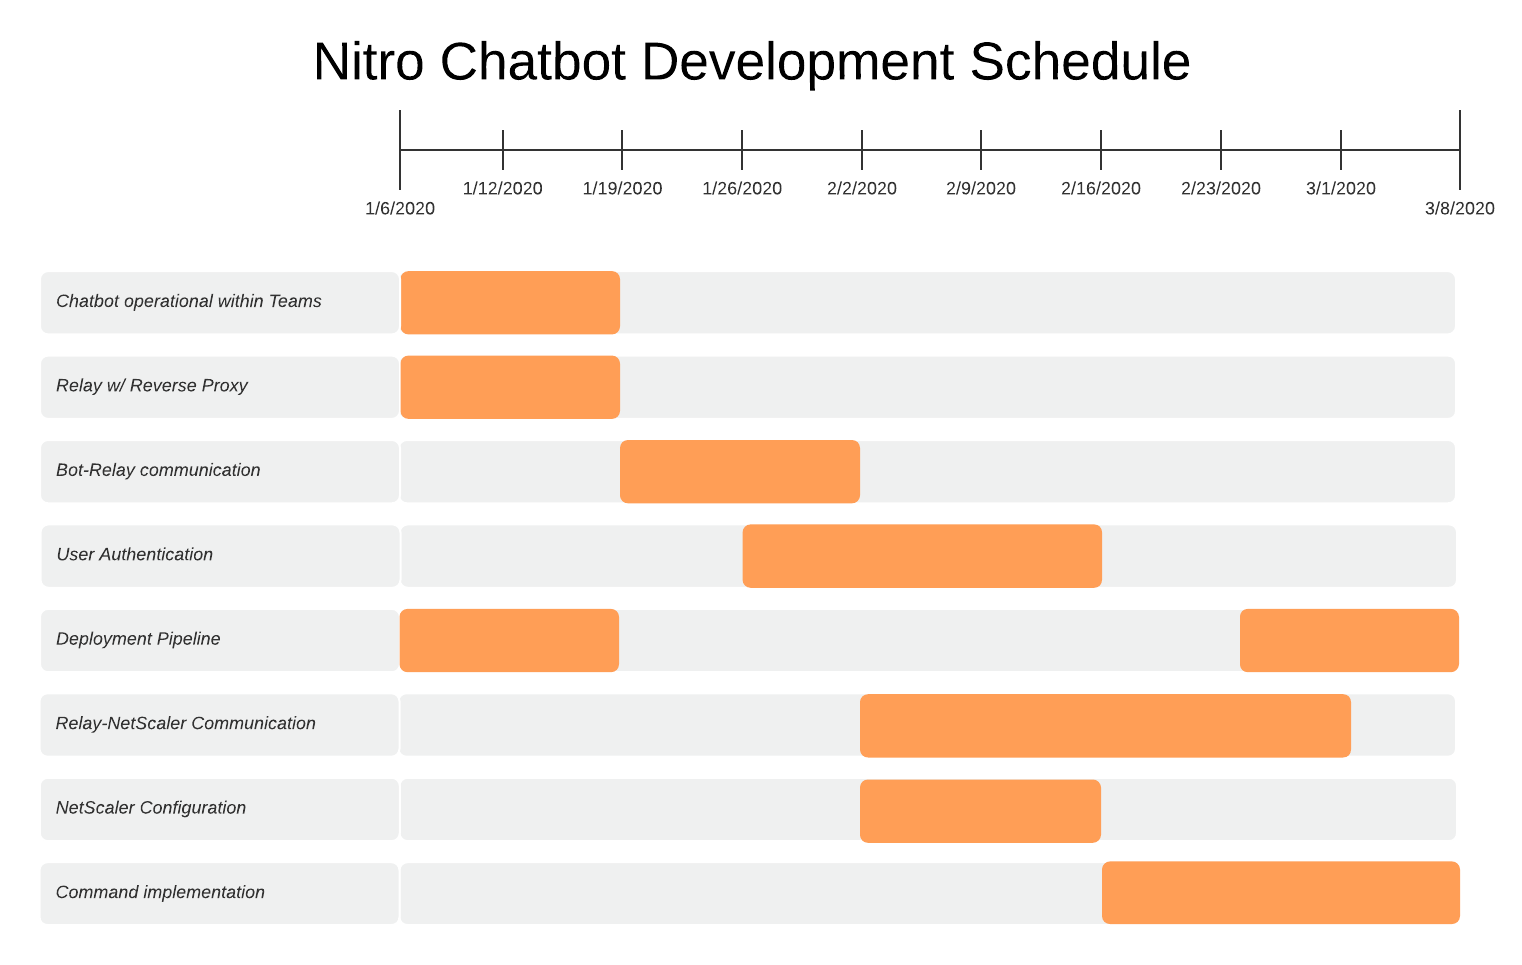
\includegraphics[height=9cm]{gantt.png}
    \caption[Feature implementation timeline]{This is tentative development schedule for Winter term 2020. This timeline give a rough estimation of when features will be implemented.}
    \label{fig:Feature implementation Timeline}
\end{figure}

\clearpage
\bibliographystyle{IEEEtran}
\bibliography{dd}
\end{document}
